\documentclass[lettersize,journal]{IEEEtran}
\usepackage{amsmath,amsfonts}
\DeclareMathOperator*{\argmin}{arg\,min}
\usepackage{algorithmic}
\usepackage{algorithm}
\usepackage{array}
\usepackage[caption=false,font=normalsize,labelfont=sf,textfont=sf]{subfig}
\usepackage{textcomp}
\usepackage{stfloats}
\usepackage{url}
\usepackage{verbatim}
\usepackage{graphicx}
\usepackage{xcolor}
\usepackage{csquotes}
\usepackage{makecell}
% my added packages and commands =======================
\usepackage[numbers]{natbib} %removed cite package

\usepackage{tikz}
\usetikzlibrary{positioning,shapes.geometric}
\usepackage{adjustbox}
\usepackage{listings}
\usepackage{caption}         

\newcommand{\highlight}[1]{\textcolor[RGB]{00,100,100}{#1}}
\newcommand{\todo}[1]{\textcolor{red}{#1}}

\captionsetup[lstlisting]{justification=centering, singlelinecheck=false}
\providecommand{\gls}[1]{#1}
\definecolor{rank1}{HTML}{70FF70}
\definecolor{rank2}{HTML}{858585}
\definecolor{rank3}{HTML}{454545}
\definecolor{rank4}{HTML}{000000}
\newcommand{\SIMSESpec}{\texttt{SIMSE\_Spec}}
\newcommand{\LoneSpec}{\texttt{L1\_Spec}}
\newcommand{\JTFS}{\texttt{JTFS}}
\newcommand{\DTWEnv}{\texttt{DTW\_Envelope}}
\newcommand{\LossSelect}{\textbf{Loss Selection}}
\newcommand{\SynthSelect}{\textbf{Synthesis Selection}}
\newcommand{\PeriodicLoss}{\textbf{Periodic Loss}}
\newcommand{\OutDomain}{\textbf{Out-Domain Generation}}
\newcommand{\BPNoise}{\textbf{BP-Noise}}  
\newcommand{\AddSineSaw}{\textbf{Add-SineSaw}}  
\newcommand{\AmpMod}{\textbf{Noise-AM}}  
\newcommand{\FMMod}{\textbf{SineSaw-AM}}  

% code_style.tex
\usepackage{xcolor}
\usepackage{tikz}

\newcommand{\greencircle}{%
    
\begin{tikzpicture}
        \fill[green] (0,0) circle (4pt); % Adjust the size here if needed
    \end{tikzpicture}%
}

\newcommand{\greenstar}{%
    
\begin{tikzpicture}[scale=0.22]
        \fill[green] 
            (0,1) 
            -- (0.2245,0.309) 
            -- (1,0.309) 
            -- (0.3633,-0.118) 
            -- (0.5878,-0.809) 
            -- (0,-0.382) 
            -- (-0.5878,-0.809) 
            -- (-0.3633,-0.118) 
            -- (-1,0.309) 
            -- (-0.2245,0.309) 
            -- cycle;
    \end{tikzpicture}%
}

\newcommand{\redcircles}{
    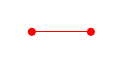
\begin{tikzpicture}[scale=0.75, line cap=round, line join=round]
        % Define coordinates for circles
        \coordinate (A) at (0,0);
        \coordinate (B) at (1,0);
        \coordinate (C) at (2,0);
        \coordinate (D) at (3,0);
        
        % Draw circles
        \foreach \point in {A,B} 
            \fill[red] (\point) circle (2pt);
        
        % Connect circles with lines
        \draw[red] (A) -- (B);
    \end{tikzpicture}%
}

\lstdefinelanguage{Faust}{
    morekeywords={import, process, environment, declare, with, if, else, while, for, int, float, true, false},
    sensitive=true,
    morecomment=[l]{//}, % Line comment
    morecomment=[s]{/*}{*/}, % Block comment
    morestring=[b]", % Strings
}

% Customize the appearance of the code
\lstset{
    language=Faust,
    backgroundcolor=\color{lightgray!20},
    basicstyle=\ttfamily\small,
    keywordstyle=\color{blue}\bfseries,
    stringstyle=\color{orange},
    commentstyle=\color{green}\itshape,
    showstringspaces=false,
    numbers=left,
    numberstyle=\tiny,
    frame=single,
    breaklines=true
}

% Suppress the "Listing #" label and caption text
% \captionsetup[lstlisting]{
%     labelformat=empty,
%     labelsep=none,
%     font=normalfont,
%     skip=0pt
% }


%  ================================
\begin{document}
\bibliographystyle{IEEEtran}


\title{Evaluating Sound Similarity Metrics for Differentiable, Iterative Sound-Matching}

\author{Amir Salimi, Abram Hindle, Osmar R. Za{\"i}ane}
\maketitle
 
\begin{IEEEkeywords}
Audio synthesis, differentiable digital signal processing, music information retrieval, sound-matching
\end{IEEEkeywords}
\hphantom{\vphantom{\begin{minipage}{\textwidth}\bibliography{references}\end{minipage}}}


% need to simplify the intro, and expand the hypothesis
\section{Introduction}
Since the 1970s, artists such as Suzanne Ciani~\cite{ciani_life_in_waves} have explored the use of audio synthesizers to replicate natural sounds—such as a bottle cap popping off—in ways that preserve the essential qualities of the original while showcasing the unique characteristics of the synthesizer~\cite{creativecherep2024}. Rather than merely replicating sounds, this approach uses synthesizers for artistic reinterpretation. However, the automation of this interpretive approach to sound design using digital audio synthesizers remains impractical for sound-designers, and significant knowledge gaps remain even in the simpler problem of replicating sounds. One such gap is the lack of diversity and depth in the analysis of sound-similarity measures and their interaction with various synthesis methods. As a stepping stone toward automated interpretive sound design, we use automatic and manual sound-evaluations to investigate whether the optimal choice of a sound-similarity measure is dependent on the synthesis method.

A digital audio synthesizer is any software used for the creation and manipulation of audio. The possibilities afforded by these synthesizers is infinite, leading to their widespread adaption by artists and sound-designers~\cite{lyons1997understanding,russ1999sound,stranneby2004digital}. A typical synthesizer has a number of parameterizable functions which affect the output sound in various ways, and the manual approach often involves modifying the parameters until a conceptualized target sound is reached. 

The automation of the aforementioned approach has been commonly referred to as "sound-matching", with reduction of tinkering time and creation of ``interesting" sounds as the main motivators \cite{krekovic2019insights,turian2020sorry,horner1993machine,salimi2020make,esling2019flow,engel2020ddsp,mitchell2007evolutionary,shier2020spiegelib,masuda2021soundmatch,masuda2023improving}. Sound-matching involves a target sound and a similarity metric (or loss function), and a heuristic to find parameters for a synthesizer that replicate \textit{all} or \textit{some} of the characteristics of a target sound as best as possible~\cite{horner1993machine,mitchell2007evolutionary,masuda2023improving}. 

We provide a review of past works in order to understand what is lacking in the field, and how it can be improved. Through our review of the history of sound-matching, we provide a nomenclature for its different subtypes, and illuminate major perennial issues that prevent sound-matching as a practical approach for sound-designers. Here we are concerned with the issues of \LossSelect~and \SynthSelect. The former refers to the search for an optimal loss function, lack of novel algorithms, and the---perhaps needless---focus on outperforming state of the art (\gls{SOTA}), while the latter refers to the lack of diversity in synthesis methods. As a consequence of these problems, we find that not much is known about the interaction between different methods of synthesis and different loss functions. We believe that clarifying the relationship between these two components is a necessary step for the prioritization of future works towards practical sound-matching. 

The main hypothesis here is that \textit{the performance of a similarity measure (or loss function) is influenced by other factors in the environment, particularly the method of synthesis}. While there have been many works and experiments comparing the accuracy of loss functions~\cite{vahidi2023mesostructures,turian2020sorry,engel2020ddsp,uzrad2024diffmoog,han2023perceptual,masuda2021soundmatch,turian2020sorry,bruford2024synthesizer}, we note that claims regarding the effectiveness of one function versus another have consistently been made in limited contexts that may not generalize to other settings; For example, it is typical for only a single (and often, simple) synthesizer to be used for testing the effectiveness of loss functions. This main hypothesis would help with important questions regarding the path of future research: Should we be searching for a universally best performing loss function across synthesizers? Does the method of synthesis influence the selection of the ``optimal" loss function, and if so, do current, SOTA loss functions satisfy the creative needs of sound-designers? 

For the experiments, an \textit{iterative} and \textit{differentiable}, approach to sound-matching is used. The iterative approach better mimics the manual process of sound design (recursively listening to synthesizer outputs and adjusting the parameters accordingly) while a differentiable environment allows access to the loss function gradients that can be used to better understand the nature of the problem. We define four differentiable synthesizers (each showcasing a fundamental method of synthesis used in modern synthesizers) and pair them with four different loss functions (two established and two novel methods). We evaluate the final similarity with two different automatic methods, as well as manual listening tests conducted by two of the authors. We compare the distributions of the evaluation scores in order to rank the loss functions from best to worst. The results of these experiments show that when accounting for different synthesizers, there is no consistent choice of sound similarity measure for optimal performance in sound-matching.


% Here, several common characteristics of previous work are avoided in order to gain fundamental, practical takeaways from the experiments. In order to directly analyze the interaction between the loss and method of synthesis, the synthesizer here are implemented with simple, functions that are used as the building blocks of complex synthesizers, and the gradients flow from the loss function to the synthesizer parameters with no extra layers between the two. Furthermore, since the true target parameters are unknown in any realistic sound-design scenario, parameter loss (P-Loss) is only used as a secondary measure of performance, and not used as a loss function.

% The simple synthesizers tested here represent fundimental building blocks of more complex implementations, and direct use of loss function gradients assuming 
%   A primary conclusion of the work is that there is no one best sound similarity measure capable of working across all synthesizers.
% The core problem that no single loss function performs optimally across synthesizer types

\section{Background and Related Works}
\subsection{Digital Audio Synthesis}
\label{sec:dsp}
A digital audio synthesizer is any software used for the creation and manipulation of digital audio. Digital synthesizers use signal processing chains with a variety of digital signal processing (\gls{DSP}) functions to create sounds. These functions are often parametric, and the set of parameters given to the synthesizer's chain of DSP functions is called a synthesizer program.

The simplest form of DSP function is a sinusoidal tone. For example, consider:
\[ x(n) = sin( 2\pi n T)\]

where $T$ represents time in seconds, and $n$ is the frequency parameter. If $n$ is 1, then $x(n)$ would be a waveform with a frequency of 1 hertz, meaning that the value of $x(n)$ oscillates to the same point once every second. Waveform generators are called oscillators for this reason. 

Since the advent of digital signal processing in the 1960s~\cite{stranneby2004digital}, a wide variety of parametric audio generation functions have been proposed~\cite{lyons1997understanding,russ1999sound,shier2020spiegelib}. This includes oscillators, filters, equalizers, and envelopes, which can be used sequentially or in parallel~\cite{lyons1997understanding,russ1999sound}. Sound design with a synthesizer is done by modifying the parameters of the functions until reaching a desired output~\cite{roads1996computer,pinch2004analog}.

Particularly in earlier works, frequency/amplitude modulators (\gls{FM}/\gls{AM}) has been the synthesizer of choice in sound-matching~\cite{horner1993machine,mitchell2007evolutionary,vahidi2023mesostructures}. This synthesis method is simple to implement, yet very expressive~\cite{chowning1973synthesis}. A common implementation is the use of one carrier, one modulator, and the corresponding envelopes:
\[ f(t) = I_c(t) \cos(\omega_c t + I_m(t) \cos(\omega_m t))
\]
Where $f(t)$ is the output signal, $I_c(t)$ is the carrier amplitude, $\omega_c$ is the carrier frequency, and $I_m(t)$ and $\omega_m$ are the envelope and frequency for the modulator~\cite{justice1979analytic}. 

Compared to the number of possible approaches to sound synthesis, a relatively small subset of synthesis methods have been analyzed in \textit{isolation} for sound-matching. Notable methods here are additive and/or subtractive synthesizers~\cite{engel2020ddsp,masuda2023improving,salimi2020make} and physical modeling~\cite{riionheimo2003parameter,han2024learning}.

\highlight{
What we mean here by \textit{isolation} is that the effect of the synthesizer's parameters (how they change the output sound and experiment outcome) is easily tractable. Recent computational advancements have allowed the use of complex Virtual Studio Technology (VST)\cite{steinberg1996vst} synthesizers in sound-matching~\cite{yee2018automatic,esling2019flow}, however, the trade-off here is the obfuscation of the interactions between the synthesizer functions, the loss, and the final outcome, among other distinctions which we will discuss in this section. 
}

An important recent development in digital audio synthesis is the increase of interest in differentiable DSP (\gls{DDSP})~\cite{engel2020ddsp}. DDSP is a general term for applications that combine machine learning techniques such as gradient descent~\cite{goodfellow2016deep,boyd2004convex} with DSP. Implementing complex DSP functions in a differentiable manner can be challenging, and effective differentiable audio similarity measures require careful mathematical expression of the desired attributes of sound. These issues have likely contributed to the limited exploration of this domain~\cite{masuda2021soundmatch,vahidi2023mesostructures,uzrad2024diffmoog}. 


\subsection{Sound Representation and Loss Functions}
\label{sec:loss_funcs}
A digital sound (or an audio signal) is a series of numbers~\cite{smith1991viewpoints,smith2007mathematics}. To compare two digital sounds, the two corresponding series are passed to a function that measures their similarity. Two signals can sound identical to our ears, without having any values in common~\cite{moore2012introduction}. This necessitates the use of proxy representations (or feature extractors) when comparing sounds automatically. Similarity between the target sound and the synthesizer output is then measured by some form of subtraction and summation of the proxy representations.

In sound-matching, particularly in a Deep Learning (\gls{DL}) context~\cite{goodfellow2016deep}, the similarity function can also be called a \textit{loss} function, where the emphasis is on measurement and reduction of the distance between target and output. It is important to note that there is a close relationship between the loss function $L$ and the sound representation function $\phi$. $L$ is the result of a distance measure $d$ applied to the features extracted by $\phi$. 

\[
L(\theta, t) = d\langle\phi(t),\phi(x)\rangle
\]

\noindent

A proxy representation is the output of the function \( \phi \), which can be thought of as a feature extraction function that maps the sounds \( t \) and \( x \) to their respective representations. 
The proportionality or distance metric $d$ has typically been the L1 distance~\cite{turian2020sorry,richard2025model}, calculated as the mean of the absolute difference between every point in the proxy representation~\cite{engel2020ddsp,vahidi2023mesostructures}:
\[
L(\theta, t) = \left\| \phi(t) - \phi(x) \right\|_1
\]

Here we discuss four methods of audio representation and the corresponding loss functions. Three of which have been used in previous works, and a novel method not previously used in iterative sound-matching. 

\subsubsection{Parameter Loss}
A common measure of similarity in sound-matching is the distance between synthesizer parameter sets, referred to as ``P-Loss"~\cite{han2023perceptual}. Typically, for the implementation of P-Loss the parameter sets are treated as vectors in space, and L1 or L2 distance is applied. There are two major limitations to this approach: First, the target and output sound must be made by the same synthesizer; otherwise the parameter sets cannot be compared (see Section~\ref{sec:matching_types}). Second, the relationship between synthesizer parameters and the audio output is not linear~\cite{shier2020spiegelib,han2023perceptual,esling2019flow}. 

\subsubsection{Fourier Spectrograms}
\label{sec:fourier_specs}
Fourier-based transformations such as short-time Fourier transforms (\gls{STFT}), Mel-spectrograms, and Mel-frequency cepstral coefficients have been viewed as the de facto and state-of-the-art representation of audio~\cite{beauchamp2003error,mitchell2007evolutionary,yee2018automatic}, however, there are many issues associated with their use in sound-matching~\cite{turian2020sorry,vahidi2023mesostructures,han2023perceptual,uzrad2024diffmoog}. Fourier transformations allow for the conversion of a signal from the time-domain to the frequency domain. Audio spectrograms can be generated by segmentation of a piece of audio into overlapping windows followed by the application of Fourier transforms to each window. They are costly to compute, but provide a better temporal view of changes in frequency content~\cite{muller2007dynamic,smith2007mathematics}. There are different types of spectrograms that have a basis in Fourier transformations, but the most notable and commonly used is the STFT.  

What we call \textit{Fourier-based Spectrograms} are variations on the STFT approach. For example, Mel-Spectrograms \textit{bin} frequencies on a near-logarithmic scale to better match human perception of frequencies~\cite{muller2007dynamic}. Multi-scale spectrograms (\gls{MSS}) used in recent works are a simple weighted average of multiple spectrograms with different parameters such as window size, number of frequency bins, and hop size~\cite{engel2020ddsp,vahidi2023mesostructures}; this may provide some improvements at a higher computational cost~\cite{turian2020sorry,engel2020ddsp}.


\subsubsection{Joint-Time Frequency Spectrum}
Recent works have focused on the limitations of parameter and spectral loss functions in sound-matching~\cite{vahidi2023mesostructures,uzrad2024diffmoog}, seeking to create more effective general solutions for the comparison of audio. 
Noting the aforementioned weaknesses of comparing STFT spectrograms, Vahidi \textit{et al.} proposed differentiable Joint-Time Frequency Scattering (\gls{JTFS})~\cite{anden2015joint} as an alternative to spectrogram loss in sound-matching, and showed improved performance in sound-matching with differentiable chirplet synthesizers~\cite{vahidi2023mesostructures}. JTFS is the result of the application of a 2D wavelet transformation to the time-frequency representation of a signal~\cite{anden2015joint}. 

\subsubsection{Dynamic Envelope Warping}
Dynamic Time Warping (DTW) is a method for measuring similarity between multi-dimensional time-series~\cite{rabiner1993fundamentals,muller2007dynamic,giorgino2009computing}. Given any two time-series $X = \{x_1,x_2,...,x_m\}$ and $Y = \{y_1,y_2,...,y_n\}$, we have indices $i\in\{1...m\}$ and $j\in\{1...n\}$ defining $X$ and $Y$. When the series are \textit{warped}, these indices change to expand or contract different portions of the series. To borrow the notation given by Muller~\cite{muller2007dynamic}, warped indices are a sequence $p=(p_1,...,p_L)$, where \(p_\ell = (m_\ell, n_\ell) \in [1 : m] \times [1 : n] \text{ for } \ell \in [1 : L]\), meaning that the indices for $X$ and $Y$ are reorganized under special conditions. In classical DTW, these conditions are \textit{monotonicity}, \textit{boundary matching}, and \textit{single step-size}.

DTW measures the distance between the time-series \textit{after} alignments, typically using Euclidean distance. The distance between a time-series and shifted versions of itself would be 0, regardless of shift amount~\cite{tavenard.blog.dtw}. Additional rules can be imposed to keep alignments locally constrained~\cite{itakura1975minimum,sakoe1978dynamic}.
% \textcolor{red}{DTW was originally used for signal comparison but using it the way we do is novel}


\subsection{Automatic Sound Matching}
\label{sec:sound_matching_definition}
The problem of sound-matching has been tackled from a variety of perspectives as it involves a number of modular parts: the choice of synthesizer $g$, the target sounds of interest, the representation function $\phi$, and the heuristic for finding the optimal $\theta$. To give a formal definition of sound-matching, we expand the definition given by recent works~\cite{vahidi2023mesostructures,han2023perceptual}. The major components are as follows: 
\begin{itemize}
    \item $g(\theta)$: Parametric audio synthesizer $g$ which takes on parameters $\theta$ 
    \item $x$: The output of $g$, given a set of parameters $\theta$ or $g(\theta) = x$ 
    \item $t$: The target sound which we want to replicate or imitate. 
    \item $\phi$: Representation function or feature extractor. $\phi$ is applied to $x$ and $t$ to facilitate their comparison by the loss function.
    \item $L$: Loss or error function. $L(\theta,t)$ is a measure of distance between $x$ and $t$. Often proportional to the subtraction of their representations, or $ \phi(x) - \phi(t)$
\end{itemize}

\highlight{It could be argued that the implementation of these components is not an optimization problem with a correct answer, but a \textit{creative} endeavor depending on the artist's needs}. Consider the hypothetical case where the goal might be to create an 8-bit~\cite{collins2007loop} version of a high quality, organic snare drum: in such a case, there is no optimal or ``correct" version of an 8-bit snare sound. 

\subsection{In-Domain versus Out-of-Domain}
\label{sec:in-domain}
The choice of domain depends on whether we want to use the same synthesizer for the target and output sounds, the scenario that is called \textit{in-domain}, or have target sounds that came from sources other than the synthesizer, or \textit{out-of-domain}. To paraphrase the description given by Masuda \textit{et al.}~\cite{masuda2021soundmatch}, if $g$, the synthesizer of choice, can accurately replicate the target sound $t$, or put differently, if $t$ itself is an output of $g$, then the sound-matching task is \textit{in-domain}. If $t$ is not an output of $g$, then the sound-matching task is \textit{out-of-domain}. In-domain tasks in general are simpler, and often there is a guarantee that there is a correct answer to the sound-matching problem, particularly if the goal is accurate replication of the sound. If the target sound is out-of-domain, replication is not guaranteed, and the goal becomes the \textit{imitation} of some aspect of sound. 

Regardless of the domain, the generation goal can be \textit{replication} or \textit{imitation} of the target sound. In replication, the goal is to make an identical copy of the target sound. Imitation is an artistic pursuit and harder to define, since the goal is to make new sounds that only retain a subset of the target's sonic features. While closely related to the in-domain versus out-of-domain problem, the choice of replication versus imitation is more dependent on how the loss and representation functions are defined. 

\subsection{Supvervised vs Direct Optimization}
\label{sec:optimization}

The choice of \textit{heuristics} is yet another important attribute sound-matching. The goal of sound-matching is to find the optimal parameters $\theta^*$ that minimize the loss between the synthesizer output and the target sound. 
\[
\theta^* = \arg\min_{\theta} L(\theta,t)
\]

The heuristics (i.e., how $\theta^*$ is approximated) used in past works can be broadly split into the two categories of \textit{direct optimization} and \textit{supervised}  (or inference) methods. Direct optimization refers to the iterative generation of a sound output, measurement of similarity between target and output, and application of updates to the parameters to maximize similarity (or minimize loss)~\cite{horner1993machine,mitchell2007evolutionary,yee2018automatic,vahidi2023mesostructures}; while supervised methods use large datasets of synthesizer sounds and corresponding parameters to learn the generation objective, commonly with the use of DNNs~\cite{engel2020ddsp,salimi2020make,yee2018automatic,esling2019flow}. These models often make their parameter predictions in a single step (or 1-shot). 

Genetic algorithms (\gls{GA})~\cite{holland1992genetic} have been the earliest and most common heuristic for direct sound-matching~\cite{horner1993machine,mitchell2007evolutionary,yee2018automatic}. These algorithms start with arbitrary parameter sets that can be treated as an evolving population where the genomes are the parameter values. The most fit members of the group are the parameters which perform the best in the loss function, and create a new generation of parameters via mutation (random change in subset of parameters) and crossovers (combination of parameter sets); this process repeats until the goal or a maximum number of generations is reached. Rather than using random mutations, differentiable approaches allow goal-oriented updates to the synthesizer parameters (the goal being the minimization of loss), but with some drawbacks: other than requiring more computation power, differentiable functions require careful implementation of operations that are continuous and numerically stable; this makes the implementation of signal processing functions quite difficult, contributing to the scarcity of works in this domain.

\subsection{Historical Framing of Sound-Matching}
Given the different attributes discussed thus far, Table~\ref{tab:summary} contains an overview of important relevant literature. This leads us to a more detailed historical analysis of past works in sound-matching.

Perhaps the earliest foundational work in sound-matching is the analytical approach by Justice~\cite{justice1979analytic} toward the decomposition and recreation of sounds using the simple FM synthesizer described in Section~\ref{sec:dsp}. The sound-matching works that followed used other heuristics for finding the synthesizer parameters, yet the simple FM synthesizer structure remained unchanged. Horner \textit{et al.}~\cite{horner1993machine} used GAs for re-synthesis of sounds with an FM synthesizer using one modulator and one carrier oscillator, and the McAulay-Quatieri method~\cite{mcaulay1986speech} for measuring loss. 


Introduction of more complex models of synthesis such as wavetables~\cite{horner2003auto} and physical modeling~\cite{riionheimo2003parameter} rendered interesting results, but led to further questions about the nature and goals of sound-matching. Mitchell and Creasy noted the difficulty in distinguishing between ``inefficiency of the optimization engine'' and ``synthesizer limitations'' as the cause of failure or success in sound-matching~\cite{mitchell2007evolutionary}. They offered a \textit{contrived methodology} for finding the best evolutionary method for sound-matching using their FM synthesizer. The methodology postulates that the best search heuristic for in-domain search (where an exact target exists, and a wide range of targets can be produced by sampling from different points in the parameter space) would also be the best-performing heuristic for out-of-domain search on a dataset of muted trumpet tones~\cite{opolko1989mcgill}; however, testing was not extensive and yielded some contradictory results. As they noted, modifications to the synthesizer, loss function, and sound domain would lead to a problem with an entirely new search space~\cite{mitchell2007evolutionary}. 

Recent years have seen more works in sound-matching using supervised machine learning techniques. In 2018, Yee-King \textit{et al.} rendered 60,000 audio-parameter pairs from the \textit{Dexed} \gls{VST} synthesizer~\footnote{https://asb2m10.github.io/dexed/}, and showed that NNs trained on this dataset can outperform GA and hill-climber (\gls{HC})~\cite{hoffmann2000heuristic} methods in rendering speed, with slight improvements in MFCC error (used as an objective performance test). The speed improvement appears trivial, considering the iterative nature of GAs when compared to offline training of supervised models. For GAs and HC optimizer, MFCCs were used as a measure of performance as well as a loss function. For training the networks, P-Loss was used, since differentiable MFCCs were not possible in their pipeline. Importantly, informal hearing tests revealed that the performance of even the best NN model was unsatisfactory, possibly due to the complex nature of the synthesizer, which features 155 parameters.

Masuda \textit{et al.} also applied supervised learning to synthesizer parameter estimation~\cite{masuda2021soundmatch}. Their work highlights the issue of non-linearity in parameter-to-synthesizer outputs and out-of-domain search. This work uses a differentiable subtractive synthesizer (two oscillators and an LP filter). A NN model was pre-trained using an in-domain dataset of randomly selected parameters and P-Loss. After training, the model was fine-tuned using 20,000 out-of-domain sounds from the NSynth dataset~\cite{engel2017neural} and multi-scale spectrogram loss~\cite{engel2020ddsp}. This approach proved more effective---i.e, achieved lower multi-level spectral difference in out-of-domain tests---than baseline models, which were either not exposed to out-of-domain sounds or trained exclusively with P-Loss. Subjective hearing tests were conducted, showing a preference for the fine-tuned model~\cite{masuda2021soundmatch}. Masuda \textit{et al.} later extended this work with semi-supervised learning, highlighting significant gaps in in-domain and out-of-domain performance~\cite{masuda2023improving}.

Rather than focusing on a particular implementation, Shier \textit{et al.} presented Spieglib, a library for implementation of sound-matching pipelines~\cite{shier2020spiegelib}. This library provides different choices for DNNs, GAs, synthesizers, and feature extractors. Shier \textit{et al.} presented an experiment with a similar setup to Yee-King \textit{et al.}~\cite{yee2018automatic}, however, they found a genetic algorithm to be the best performing.

Differentiable loss functions that use spectrogram differences can be computationally expensive. To mitigate this, Han \textit{et al.}~\cite{han2023perceptual} introduced ``perceptual-neural-physical loss'' (PNP). PNP is an approximation of loss functions; specifically, a loss function that uses the L2 norm of the difference between the features of two sounds, or $||\phi(t) - \phi(x)||^2_2$, where $\phi$ could be a spectrogram or JTFS function. PNP loss functions are fast and differentiable, but require training and parameter estimation. A Riemannian metric M needs to be calculated for the minimization of locally linear approximation of the ``true" spectral loss function~\cite{han2023perceptual}. 
\[
\|\phi(t) - \phi(x)\|_2^2 = \langle \tilde{\theta} - \theta | \mathbf{M}(\theta) | \tilde{\theta} - \theta \rangle + O(\|\tilde{\theta} - \theta\|_2^3). \tag{4}
\]

During the training phase, this metric is calculated alongside the neural parameter estimator. After training, PNP can be used as a fast approximation of computationally demanding loss functions such as JTFS~\cite{han2023perceptual,han2024learning}, paired with FM synthesizers and a differentiable physical model of a drum head~\cite{smith2010physical}.

A neural approximation for another part of the supervised sound-matching chain---this time the synthesizer---was proposed by Barkan \textit{et al.}~\cite{barkan2023inversynthII}. As they noted, without a differentiable synthesizer, ``model-based'' (or what we call supervised) approaches cannot directly compare $x_o$ to $x_t$, often opting for P-Loss, which may not correctly map the parameters of sound to the output audio~\cite{esling2019flow,han2023perceptual,masuda2023improving}. Given a synthesizer and a large dataset of sounds and corresponding parameters, a model which maps sounds to parameters, and another model which approximates the synthesizer can be trained, allowing the implementation of a loss function which combines P-Loss with STFT differences. This ``Inversynth II'' (IS2) approach yielded significant improvements to previous works which did not use the STFT approximations for loss~\cite{esling2019flow,barkan2019inversynth}.

Barkan \textit{et al.} attemped to  improve the IS2 model with Inference-Time
Finetuning (ITF). For ITF, the synthesizer approximation is frozen and the encoder is iteratively finetuned for the sample sample using gradient descent in order to minimize P-Loss, stopping at convergence or when maximum number of iterations has reached~\cite{barkan2023inversynthII}. Barkan \textit{et al.} report that perhaps due to the discrepancy between the true and approximated synthesizer or overfitting, the application of ITF to IS2 generally worsened the spectral and manual performance metrics.


Uzrad \textit{et al.}~\cite{uzrad2024diffmoog} took another unique approach to sound-matching: using a differentiable \textit{synthesis chain} of DSP generators and effects and a loss function that combines P-Loss with a \textit{signal-chain loss}. The synthesizer is a customizable chain of effects, which feed one output as input to the next step of the chain; signal-chain loss compares the parameter and output difference at every output step in the chain~\cite{uzrad2024diffmoog}. Possible chain functionalities are FM/AM, Low-Frequency Oscillators (\gls{LFO}), filters, and envelopes. Like the results shown by Masuda \textit{et al.}~\cite{masuda2021soundmatch}, better out-of-domain results were achieved when pre-trained on in-domain data and fine-tuned using out-of-domain NSynth data~\cite{engel2017neural}.


Some recent works have opted for the use of audio embeddings as a similarity metric. In a recent work, Cherep \textit{et al.} used latent representations from the CLAP model~\cite{wu2023large} along with a differentiable synthesizer~\cite{synthhaxcherep2023} to create creative interpretations of sound effects. In their approach, a desired sound-effect is described in text and embedded using clap, and gradient free optimizer~\cite{evosax2022github} iteratively updates the synthesizer's parameters to minimize difference in the text and output sound embeddings. Based on manual hearing tests, this approach did not produce the ``correct'' sounds more frequently than previous works~\cite{kreuk2022audiogen}, however, it did yield better scores for ``artistic-interpretation'' (or what we refer to as imitation). 


% masuda and esling both noted out-of-domain drop in performance
% yee king noted performance drop in manual surveys 
%p-loss bad : masuda-improving, han2023, esling-flowsynth
% manual performance measure: barkan, masuda2021soundmatch, yee-king 

\end{document}


